\documentclass[border=20pt]{standalone}
\renewcommand\familydefault{\sfdefault} % Default family: serif 
\usepackage[usenames,dvipsnames]{xcolor}
\usepackage{tikz}
%\usepackage{soul}
\usetikzlibrary{calc} 
\usetikzlibrary{arrows, decorations.markings,positioning,backgrounds,shapes}
\usetikzlibrary{patterns}
\usetikzlibrary{fit}
\usepackage[normalem]{ulem}

\begin{document}
	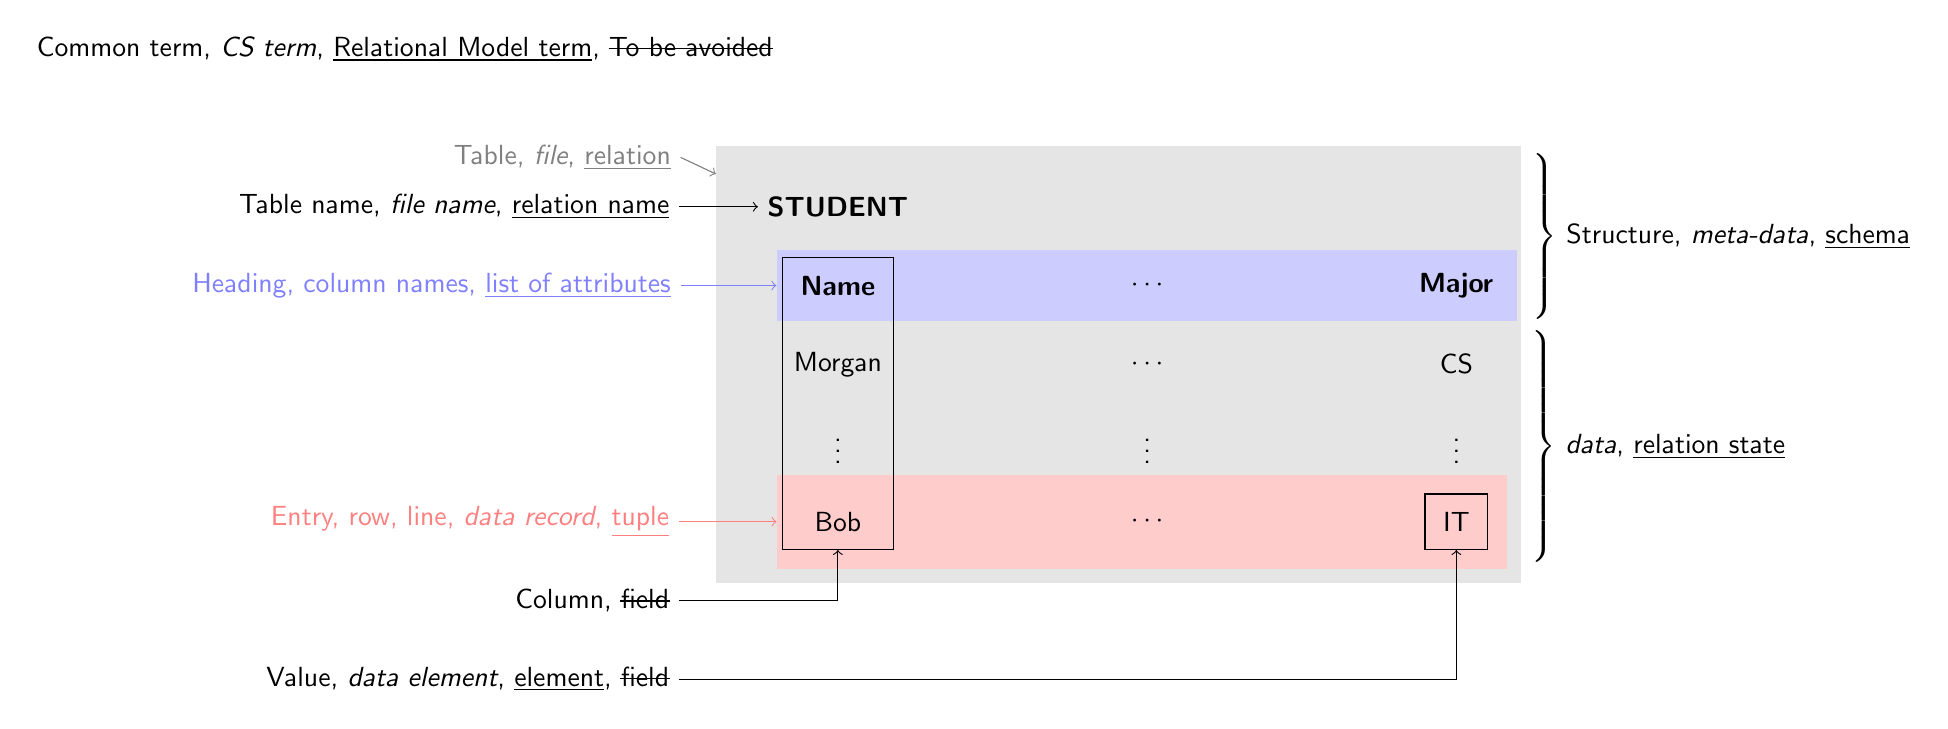
\begin{tikzpicture}
	% Caption:
	\node (caption) at (-5.5,2) {	Common term, \emph{CS term}, \underline{Relational Model term}, \sout{To be avoided}};
	
	% Table:
	\node (name) {\textbf{STUDENT}};
	\node [below of=name] (Name) {\textbf{Name}};
	\node [right= 3 of Name] (dots1) {\(\cdots\)};
	\node [right= 3 of dots1] (Major) {\textbf{Major}};
	\node [below of= Name] (Morgan) {Morgan};
	\node [below of= dots1] (dots2) {\(\cdots\)};
	\node [below of= Major] (CS) {CS};
	\node [below of= Morgan] (dots3) {\(\vdots\)};
	\node [below of= dots2] (dots4) {\(\vdots\)};
	\node [below of= CS] (dots5) {\(\vdots\)};
	\node [below of= dots3] (Bob) {Bob};
	\node [below of= dots4] (dots6) {\(\cdots\)};
	\node [below of= dots5] (IT) {IT};
	% Annotations:
%	\draw [-, dashed] (-1.5, 0.75) -- ++ (11,0);
%	\draw [-, dashed] (-1.5, -1.45) -- ++ (11,0);
	\node (meta) at (11.2, -0.35) {\(\left.\rule{0cm}{1.2cm}\right\}\) Structure, \emph{meta-data}, \underline{schema}};
	\node (data) at (10.4, -3.0) {\(\left.\rule{0cm}{1.65cm}\right\}\)  \emph{data}, \underline{relation state}};
	\begin{scope}[on background layer]
		\node [fit=(name)(IT), fill=gray!20, draw = none, inner sep= 15pt] (box1) {};	
		\node [fit=(Name)(Major), fill=blue!20, draw = none, inner sep= 5pt] (box2) {};	
		\node [fit=(Bob)(IT), fill=red!20, draw = none, inner sep= 10pt] (box3) {};	
		\node [fit=(Name)(Bob), draw = black, inner sep= 3pt] (box4) {};	
		\node [fit=(IT), draw = black, inner sep= 3pt] (box5) {};	
				
%		\draw [fill=gray!20, draw=none] (IT)+(1,-0.5) rectangle (name.north west);
%		
		%
%		\draw [fill=blue!20, draw=none] (Bob)+(0.6,-0.2) rectangle  (Name.north west);
%		\draw [pattern=north west lines, pattern color=blue!40, draw=none] (Bob)+(0.6,-0.2) rectangle  (Name.north west);
%		\draw [] (Major.south east) rectangle  (Name.north west);
%		\draw [] (CS.south east) rectangle  (Morgan.north west);
%		\draw [] (IT.south east) rectangle  (IT.north west);
%		\node[inner sep=10pt,draw,fit=(IT)] (box) {};
%		\node [fit=(Bob)(Name)(Bob)(Name), fill=blue!20] () {};
	\end{scope}
	
	\node (names) [left = 1cm of name] {Table name, \emph{file name}, \underline{relation name}};
	\draw[->] (names) -- (name);
	\node (Table) [above = 0.1 of name, xshift = -3.5cm]{\textcolor{gray}{Table, \emph{file}, \underline{relation}}};
	\draw[->, bend right=-80, gray] (Table.east) -- (box1);
	\node (header) [left = 1.4cm of Name] {\textcolor{blue!50}{Heading, column names, \underline{list of attributes}}};	
	\draw[->, blue!50] (header) -- (box2);

%	\node (acc) [left = 0.9cm of names, yshift = -0.4cm] {Meta-data \(\left\{\rule{0cm}{0.9cm}\right.\)};	
	
	\node (entry) [left = 1.6cm of Bob] {\textcolor{red!50}{Entry, row, line, \emph{data record}, \underline{tuple}}};
	\draw[->, red!50] (entry) -- (box3);
	
	\node (column) [left = 1.6cm of Bob, yshift=-1cm] {Column, \sout{field}};
	\draw[->] (column) -| (box4);
	
	\node (value) [left = 1.6cm of Bob, yshift=-2cm] {Value, \emph{data element}, \underline{element}, \sout{field}};
	\draw[->] (value) -| (box5);
	\end{tikzpicture}
	

\end{document}